\chapter{Sistema biometrico: elementi caratteristici}

\section{Struttura di un sistema biometrico}

\subsection{Struttura di un sistema biometrico (generale)}

\subsubsection{Fase di enrollment}

\begin{figure}[ht]
    \centering
    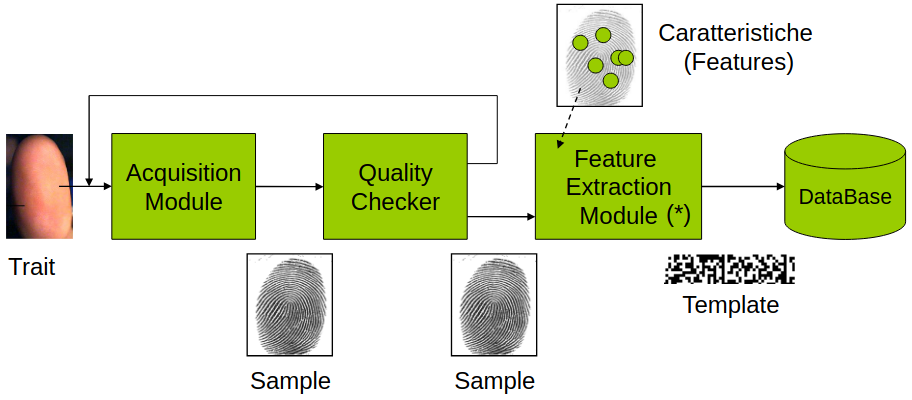
\includegraphics[width=0.95\linewidth]{chapters/images-chap2/enrollment-gen.png}
    \caption{Enrollment: (template) --$>$ DB}
    \label{fig:enroll-gen}
\end{figure}

\begin{figure}[ht]
    \centering
    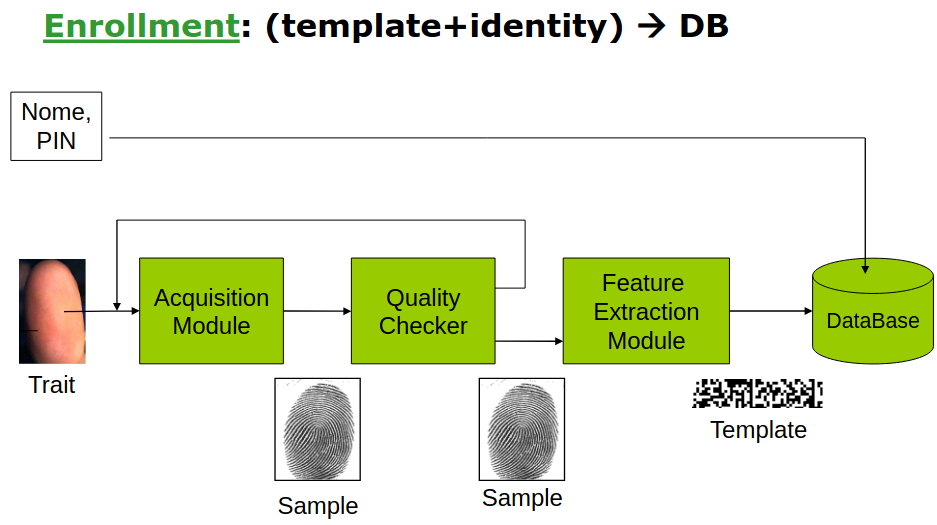
\includegraphics[width=0.95\linewidth]{chapters/images-chap2/enrollment-gen-id.png}
    \caption{(template + identity) --$>$ DB}
    \label{fig:enroll-gen-id}
\end{figure}

\newpage

\subsubsection{Verification usando un DB}

\begin{figure}[ht]
    \centering
    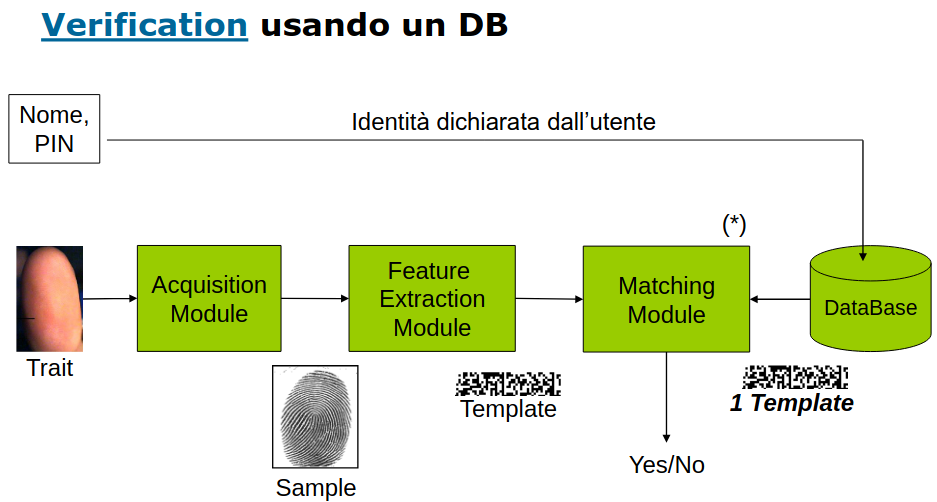
\includegraphics[width=0.95\linewidth]{chapters/images-chap2/verification-gen.png}
    \caption{Verification usando un DB}
    \label{fig:verification-gen}
\end{figure}

\newpage
\subsubsection{Identification}

\begin{figure}[ht]
    \centering
    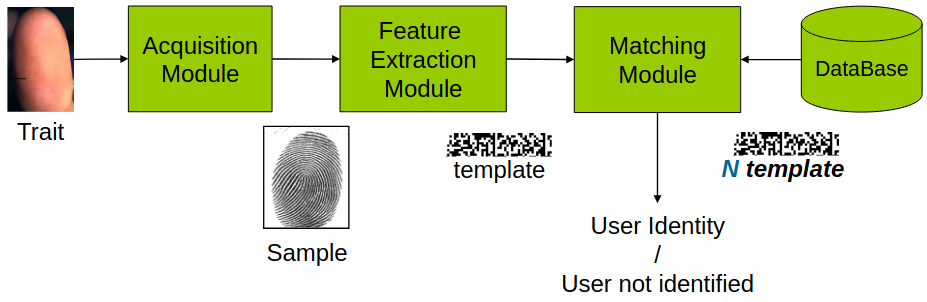
\includegraphics[width=0.95\linewidth]{chapters/images-chap2/identification-gen.png}
    \caption{Identification}
    \label{fig:id-gen}
\end{figure}

\subsection{Struttura per documenti biometrici}

\subsubsection{Fase di enrollment}

\begin{figure}[ht]
    \centering
    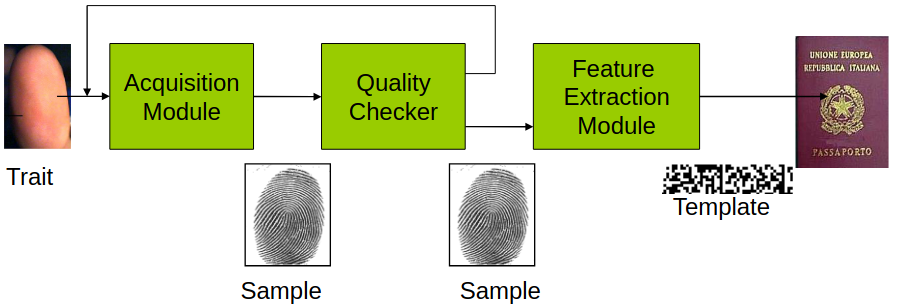
\includegraphics[width=0.95\linewidth]{chapters/images-chap2/enroll-doc.png}
    \caption{(template) --$>$ Documento}
    \label{fig:enroll-doc}
\end{figure}

\newpage
\subsubsection{Verification (con documento biometrico)}

\begin{figure}[ht]
    \centering
    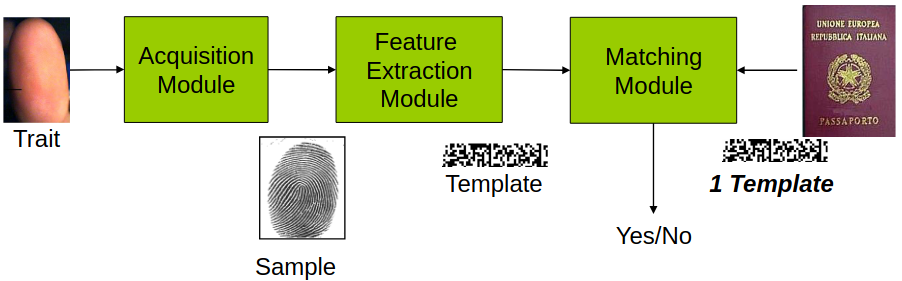
\includegraphics[width=0.95\linewidth]{chapters/images-chap2/verification-doc.png}
    \caption{Verification con documento biometrico}
    \label{fig:enter-label}
\end{figure}

\subsection{Struttura dei sistemi multimodali}

\begin{figure}[ht]
    \centering
    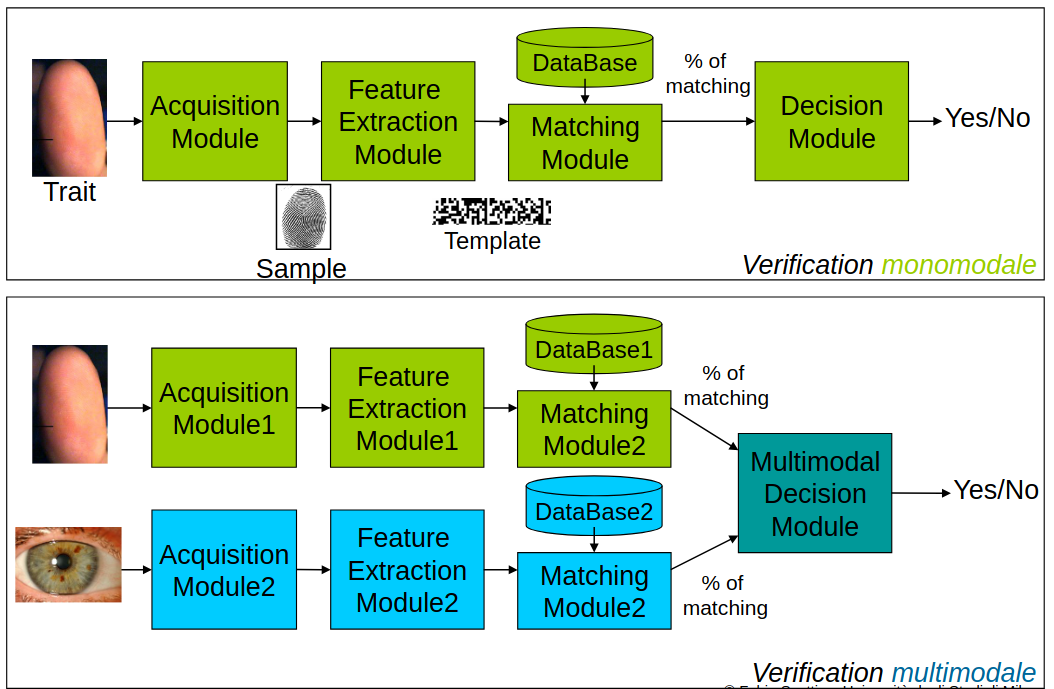
\includegraphics[width=0.95\linewidth]{chapters/images-chap2/multimodali.png}
    \caption{Confronto tra la struttura di un sistema monomodale e multimodale}
    \label{fig:multimodal}
\end{figure}

\subsection{Struttura dei sistemi biometrici distribuiti}

Il termine “distribuito” si riferisce ad un sistema biometrico quando i moduli componenti sono separati e collegati in rete.
Piuttosto raro quando si parla di sistemi di autenticazione; è invece comune quando si parla di sistemi di identificazione di grosse dimensioni. 


Solitamente è il modulo dei database ad essere separato dai terminali.
\begin{figure}[ht]
    \centering
    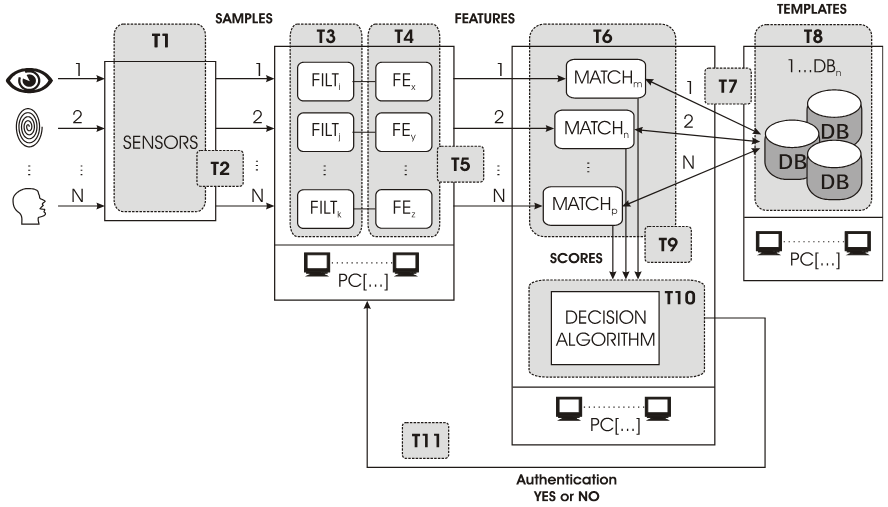
\includegraphics[width=0.95\linewidth]{chapters/images-chap2/distributed.png}
    \caption{Struttura di un sistema biometrico distribuito}
    \label{fig:distr}
\end{figure}

\subsection{Sistemi biometrici on card}
Il termine on card si riferisce al fatto che il template biometrico risiede su una smart card.

\newpage

\section{Tratto biometrico: aspetti analitici}

\subsubsection{Variabilità intraclasse}

Si intende la variazione del \textbf{sample} o delle \textbf{feature} dello stesso individuo tra acquisizioni effettuate in istanti di tempo diversi.
Può essere dovuto a:
\begin{itemize}
    \item effetti casuali (rumore del dispositivo)
    \item varizioni dello sfondo
    \item variazioni del tratto (invecchiamento, posizione, espressioni, ecc.)
\end{itemize}

\subsubsection{Similitudine interclasse}

Particolare vicinanza dei \textbf{sample} o delle \textbf{feature} acquisiti da individui diversi.

\section{Regole Generali di Progettazione}

\subsection{Acquisizione del tratto}

Analizziamo i metodi per \textbf{progettare} ed eventualmente \textbf{migliorare} il modulo di acquisizione.

L'acquisizione di una informazione rilevante \textbf{è un processo critico} e non sempre adeguatamente studiato.

La cura nel processo di acquisizione \textbf{influenza pesantemente l'accuratezza} finale del sistema.

Il processo di acquisizione si divide in \textbf{due fasi:}
\begin{itemize}
    \item \textbf{Valutazione della qualità:} controllo automatico sulla correttezza dei dati in ingresso coerentemente alle successive elaborazioni
    \item \textbf{Segmentazione:} separazione dei dati in ingresso nell'oggetto di interesse (foreground) e nello sfondo/informazione non rilevante (background)
\end{itemize}

\subsubsection{Estrarre molte informazioni}

È buona prassi cercare di estrarre maggiori informazioni possibili per migliorare le performance del sistema biometrico.
\begin{itemize}
    \item \textbf{Acquisire anche il contesto} attorno al sample; permette di trovare meglio il vero volto per sottrazione di frame senza elaborazioni troppo complesse
    \item \textbf{Evitare sul nascere di fare cattive acquisizioni} per non dover richiedere il sample (ad esempio, controllare se il soggetto è in movimento o alla distanza corretta prima di elaborare il frame)
\end{itemize}

\subsection{Controllo della qualità}

Dopo l'acquisizione molti sistemi attuano un controllo automatico della qualità del tratto rilevato per evitare problemi di funzionamento.

I sistemi di controllo della qualità producono un \textbf{indice di qualità} del sample acquisito:
\begin{itemize}
    \item se l'indice di qualità è sufficientemente alto si prosegue
    \item altrimenti si torna ad acquisire un altro sample
\end{itemize}

Il concetto di base è semplice, ma la progettazione e realizzazione dell'indice di qualità non lo è; alcuni punti sono che:
\begin{itemize}
    \item non sempre esiste un \textbf{modello rigoroso e realistico} della misura in ingresso da usare per calcolare l'indice; ad esempio, se potessimo definire come dovrebbe essere un'immagine ottimale di un'impronta, potremmo esprime l'indice di qualità come la "distanza" dell'immagine in ingresso da quella ottima
    \item non sempre esistono \textbf{metriche rigorose e robuste} per misurare la distanza del sample in ingresso con il riferimento ottimale
\end{itemize}

\subsection{Signal/Image enhancement}
In alcuni casi non è possibile rifiutare un sample perché il suo indice di qualità è basso (ad esempio database giudiziari); in questo caso, il sistema cerca di estrarre le informazioni (foreground) dal rumore (background) in modo tale da far funzionare il resto della catena di moduli del sistema.

Solitamente questa fase è ad alta complessità computazionale. Può generare i cosidetti \textbf{artefatti}; ad esempio, data un'impronta rumorosa genere delle minuzie che non erano presenti nell'immagine originale.

